\documentclass{article}%
\usepackage[T1]{fontenc}%
\usepackage[utf8]{inputenc}%
\usepackage{lmodern}%
\usepackage{textcomp}%
\usepackage{lastpage}%
\usepackage[head=40pt,margin=0.5in,bottom=0.6in]{geometry}%
\usepackage{graphicx}%
%
\title{\textbf{Dictaron privativa de libertad para presidente de la FCU de la UC}}%
\author{El Nacional Web}%
\date{07/11/2018}%
%
\begin{document}%
\normalsize%
\maketitle%
\textbf{URL: }%
http://www.el{-}nacional.com/noticias/politica/dictaron{-}privativa{-}libertad{-}para{-}presidente{-}fcu\_258954\newline%
%
\textbf{Periodico: }%
EN, %
ID: %
258954, %
Seccion: %
Política\newline%
%
\textbf{Palabras Claves: }%
NO\_TIENE\newline%
%
\textbf{Derecho: }%
1.2%
, Otros Derechos: %
1.10%
, Sub Derechos: %
1.2.2, 1.10.1%
\newline%
%
\textbf{EP: }%
NO\newline%
\newline%
%
\textbf{\textit{Pablo Aure, secretario general de la Universidad de Carabobo (UC), rechazó la medida}}%
\newline%
\newline%
%
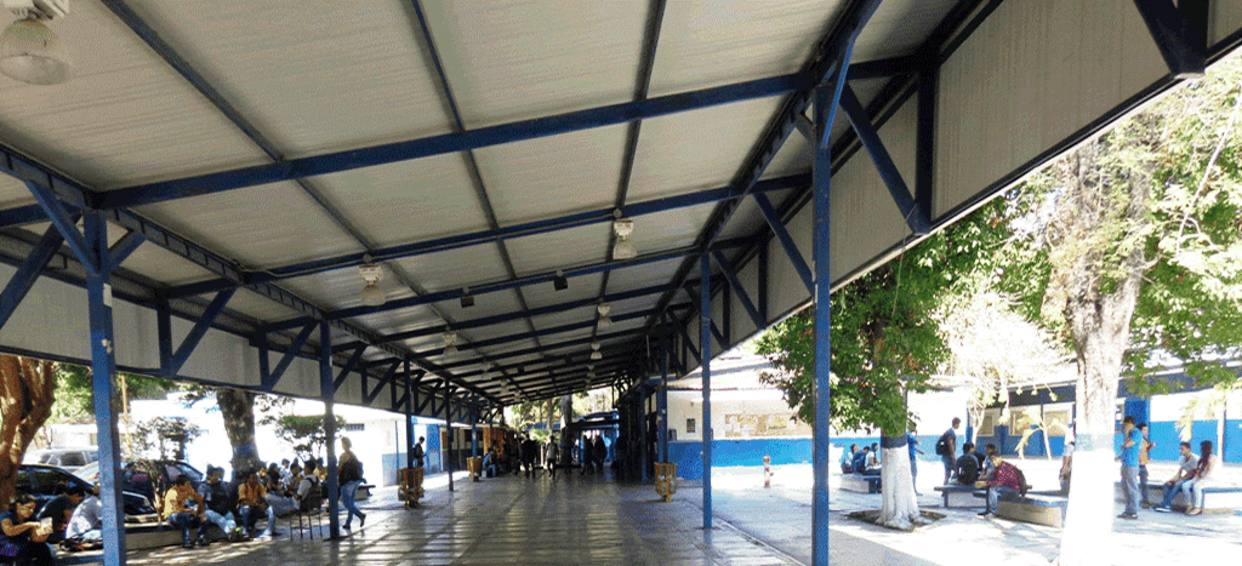
\includegraphics[width=300px]{36.jpg}%
\newline%
%
Pablo Aure, secretario general de la Universidad de Carabobo (UC), informó este miércoles que se dictó privativa de libertad para Ivan Uzcátegui, presidente de la Federación de Centros Universitarios de la UC; y para Ramón Bravo , director de comedores de la casa de estudio.%
\newline%
%
"Acaba de salir audiencia de presentación de Ivan Uzcátegui, presidente FCU{-}UC y de Ramon Bravo,~director de Comedores UC.~El Tribunal de control decretó medida privativa de libertad", escribió en su Twitter.%
\newline%
%
Aure catalogó el hecho como una injusticia y aseguró que es una medida en contra de la universidad. "Siguen cometiendo injusticia. Atacando la Universidad. La UC no se rendirá".%
\newline%
%
Noticia en desarrollo%
\newline%
%
\end{document}